% !TeX spellcheck = ru_RU-Russian
\documentclass[14pt]{article}
\usepackage[14pt]{extsizes}
\usepackage[utf8]{inputenc}
\usepackage[T2A]{fontenc}
\usepackage[english, russian]{babel}
\usepackage[a4paper,left=20mm, right=10mm, top=20mm, bottom=20mm]{geometry}
\usepackage{indentfirst, setspace}
\setlength{\parindent}{1.25cm}
\usepackage{tabularx, multirow}
\usepackage[normalem]{ulem}
\usepackage[style=russian]{csquotes}
\usepackage{ragged2e}

% Font setup for PDF compatibility
\usepackage{cmap}
\usepackage{graphicx}
\usepackage{wrapfig}
\graphicspath{ {images/} }

\fontsize{12}{12}\selectfont
\usepackage{amsmath,amsfonts,amssymb}
\usepackage{mathtools}
\usepackage{listings}
\usepackage[center]{caption}
\renewcommand{\labelenumii}{\arabic{enumi}.\arabic{enumii}.}
\renewcommand{\labelenumiii}{\arabic{enumi}.\arabic{enumii}.\arabic{enumiii}.}
\renewcommand{\labelenumiv}{\arabic{enumi}.\arabic{enumii}.\arabic{enumiii}.\arabic{enumiv}.}
\DeclareCaptionLabelSeparator{custom}{ --- }
\captionsetup{labelsep=custom}
\usepackage{pgfplots}
\usepackage{pdfpages}
\pgfplotsset{compat=1.9}
\usepackage{xcolor}
\usepackage{hyperref}
\definecolor{linkcolor}{HTML}{000000} 
\definecolor{urlcolor}{HTML}{000000} 
\hypersetup{pdfstartview=FitH,linkcolor=linkcolor,urlcolor=urlcolor, colorlinks=true}
\captionsetup[figure]{name=Рисунок}


\begin{document}
	
	\thispagestyle{empty}
	
	\noindent \begin{minipage}{0.15\textwidth}
		\includegraphics[width=\linewidth]{1}
	\end{minipage}
	\noindent\begin{minipage}{0.85\textwidth}\centering
		\textbf{Министерство науки и высшего образования Российской Федерации}\\
		\textbf{Федеральное государственное бюджетное образовательное учреждение высшего образования}\\
		\textbf{«Московский государственный технический университет имени Н.Э.~Баумана}\\
		\textbf{(национальный исследовательский университет)»}\\
		\textbf{(МГТУ им. Н.Э.~Баумана)}
	\end{minipage}
	
	\noindent\rule{\linewidth}{3pt}
	\newline\newline
	\noindent ФАКУЛЬТЕТ $\underline{\text{«ФУНДАМЕНТАЛЬНЫЕ НАУКИ»}}$ \newline\newline
	\noindent КАФЕДРА $\underline{\text{«ПРИКЛАДНАЯ МАТЕМАТИКА»}}$
	
	\vspace{1cm}
	
	\begin{center}
		\noindent\centering
		\Large\textbf{Лабораторная работа № 1}
		
	\end{center}
	\begin{center}
		\noindent\centering
		\Large\textbf{по дисциплине <<Типы и структуры данных>>}
	\end{center}
	
	\noindent\textbf{Тема} $\underline{\text{Умножение мартиц}}$\newline\newline
	\noindent\textbf{Студент} $\underline{\text{Лямин И.С.}}$\newline\newline
	\noindent\textbf{Группа} $\underline{\text{ФН12-31Б}}$\newline\newline
	\noindent\textbf{Преподаватели} $\underline{\text{Волкова Л.Л.}}$\newline
	
	\begin{center}
		\vfill
		Москва,~\the\year 
	\end{center}
	\clearpage
	

	\renewcommand{\contentsname}{\centering{СОДЕРЖАНИЕ}}
	\setcounter{page}{2}
	\tableofcontents
	
	\newpage
	\begin{center}
		\section*{ВВЕДЕНИЕ} 
	\end{center}
	
	В лабораторной работе будут разобраны и реализованы алгоритмы перемножения произвольных матриц(отличных рамеров), стандартным алгоритмом, алгоритмом Винограда и оптимизированным алгоритмом Винограда.
	
	Во всей работе подразумевается, что $lh$(left height) -- высота левой матрицы, $lw$(left wide) -- ширина левой матрицы, $rh$(right height) -- высота правой матрицы, $lh$(right wide) -- ширина правой матрицы.   
	
	\textbf{Цель работы } -- выполнить оценку ресурсной эффективности алгоритмов перемножения мартиц и их реализации.\par
	Для достижения поставленной цели требуется выполнить следующие задачи.
	\begin{enumerate}
		\item Описать математическую основу обычного алгоритма, алгоритма Винограда и оптимизированного алгоритма Винограда перемножения стриц,
		\item Описать модель вычисления,
		\item Реализовать программу на основе этих алгоритмов.
		\item Выполнить оценку трудоёмкости реализации алгоритмов,
		\item Реализовать разработанные алгоритмы в программном обеспечении с двумя режимами работы -- одиночного расчёта и массированного замера процессорного времени,
		\item Выполнить замеры процессорного времени выполнения реализации каждого алгоритма в зависимости от размера матриц,
		\item Выполнить сравнительный анализ рассчитанных трудоёмкостей и результатов замера процессорного времени,
	\end{enumerate}
	
	\newpage
	\section{Аналитическая часть}
	
	\subsection{Стандартный алгоритм}
	\textbf{Стандартный алгоритм:} представляет собой поочёрёдное перемножение i-ой вектор-строки первой мартицы на j-ый вектор-столбец второй матрицы, таким образом получим элемнт [i, j] из матрицы. Формула для этого метода перемножения выглядит следующим образом:
	\begin{equation*}
		A = \left(
		\begin{array}{cccc}
			a_{11} & a_{12} & \ldots & a_{1m}\\
			a_{21} & a_{22} & \ldots & a_{2m}\\
			\vdots & \vdots & \ddots & \vdots\\
			a_{n1} & a_{n2} & \ldots & a_{nm}
		\end{array}
		\right)
		B = \left(
		\begin{array}{cccc}
			b_{11} & b_{12} & \ldots & b_{1l}\\
			b_{21} & b_{22} & \ldots & b_{2l}\\
			\vdots & \vdots & \ddots & \vdots\\
			b_{m1} & b_{m2} & \ldots & b_{ml}
		\end{array}
		\right)
	\end{equation*}
	\begin{equation}
		A*B_{i,j} = \sum_{k=1}^m (a_{ik} \cdot b_{kj})
	\end{equation}
	
	\subsection{Алгоритм Винограда}
	\textbf{Алгоритм Винограда} --- алгоритм направлен на уменьшение количества операций умножения помещением часто используемых произведений в буффер и использованием вычисленных значений при необходимой итерации. Рассмотрим элемент  $c_{ij}$ из матрицы $C$:
	\begin{equation}
		c_{ij} = \sum_{k=1}^{m/2} ((a_{ik\cdot 2} + b_{k\cdot 2 + 1j})\cdot (a_{ik\cdot 2+1} + b_{k\cdot 2j}) -
		(a_{ik\cdot 2}\cdot a_{ik\cdot 2+1}) - (b_{ik\cdot 2}\cdot b_{ik\cdot 2+1}))
	\end{equation}
	На этом тождестве основывется алгоритм Винограда. Все произведения вида $a_{i,k}*a_{i,k+1}$, будут всегда вычитаться при получении элемента $i$-ой строки новой матрицы и аналогично $j$-ого столбца. Следовательно можно создать два массива с элементами которые используются по одному при каждой итерации вычисления значения элемента матрицы $c_{i,j}$.
	\begin{gather}
		rows[j] = \sum_{i=0}^{m/2} (a_{ji\cdot2}\cdot a_{ji\cdot 2+1}), j=1,2,3,...,n,\\
		\begin{gathered}
			columns[j] = \sum_{i=0}^{n/2} (b_{i\cdot
				2j}\cdot b_{i\cdot 2+1j}),j=1,2,3,...,l
		\end{gathered}
	\end{gather}
	где $m$ - количество стлобцов первой матрицы,\\
	$n$ - количество строк в первой матрице, $l$ - количество столбцов во второй матрице
	
	Итоговая формула вычисления значений элемента строки $i$ столбца $j$ матрицы $C$ имеет вид:
	\begin{equation}
		c_{ij} = (\sum_{k=1}^{m/2} (a_{ik\cdot 2} + b_{k\cdot 2 + 1j})\cdot (a_{ik\cdot 2+1} + b_{k\cdot 2j})) - row[i] - columns[j]
	\end{equation}
	И для случая когда $m$ нечётное:
	\begin{equation}
		c_{ij} = (\sum_{k=1}^{(m-1)/2} (a_{ik\cdot 2} + b_{k\cdot 2 + 1j})\cdot (a_{ik\cdot 2+1} + b_{k\cdot 2j})) - row[i] - columns[j] + a_{i(m/2)}\cdot b_{(m/2)j}
	\end{equation}
	
	\subsection{Оптимизированный алгоритм Винограда}
	\textbf{Оптимизированный Алгоритм Винограда} --- оптимизация моего варианта состоит в замене операции умножения на двоичный сдвиг:
	\begin{gather}
		c_{ij} = (\sum_{k=1}^{(m)/2} (a_{ik<<1} + b_{k<<1 + 1j})\cdot (a_{ik<<1+1} + b_{k<<1j})) - row[i] - columns[j]\\
		\begin{gathered}
			c_{ij} = (\sum_{k=1}^{(m-1)/2} (a_{ik<<1} + b_{k<<1 + 1j})\cdot (a_{ik<<1+1} + b_{k<<1j}))\\
			- row[i] - columns[j] + a_{i(m/2)}\cdot b_{(m/2)j}
		\end{gathered}
	\end{gather}
	формула (7) для случая чётного количество строк в первой матрице и формула (8) для нечётного случая.
	
	Второй частью оптимизации было объединение операции нахождения массивов $rows$ и $columns$. Реализовано следующим образом, $lim=max(l_w, r_h)$, где $l_w$-ширина левой матрицы, а $r_h$-высота правой. Пременная $lim$ показывает до какой итерации дойтёт цикл в котором будут перемножаться $i$ и $i + 1$ элементы из соответствующий строк и столбцов. И в момент когда либо строки в первой матрице, либо столбцы во второй закончатся, то перемножение элементов строки или соответственно столбца прекратится, а процесс получения второго массива продолжится до момента пока количество интераци не достигнет значения lim. Это будет реализованно в коде, также как и вынос первой итерации.
	\newpage
	
	\section{Конструкторская часть}
	\subsection{Описание алгоритмов}
	На следующих рисунках блок-схем представлены соответствующие алгоритмы:~\ref{fig:label2} - стандартный алгоритм, ~\ref{fig:label5} - Алгоритм Винограда, и оптимизированный алгоритм Винограда ~\ref{fig:label6}. Также перед описанием алгоритма Винограда и оптимизированного алгоритма Винограда опишем вспомогательные функции $prepair\_arrays$ рисунок ~\ref{fig:label3} и $optimzed\_prepair\_arrays$ рисунок ~\ref{fig:label4}
	
	\begin{center}
		
		\includegraphics[width = 0.85\textwidth]{diagram_2}
		\captionof{figure}{Схема стандартного алгоритма}
		\label{fig:label2}
		
		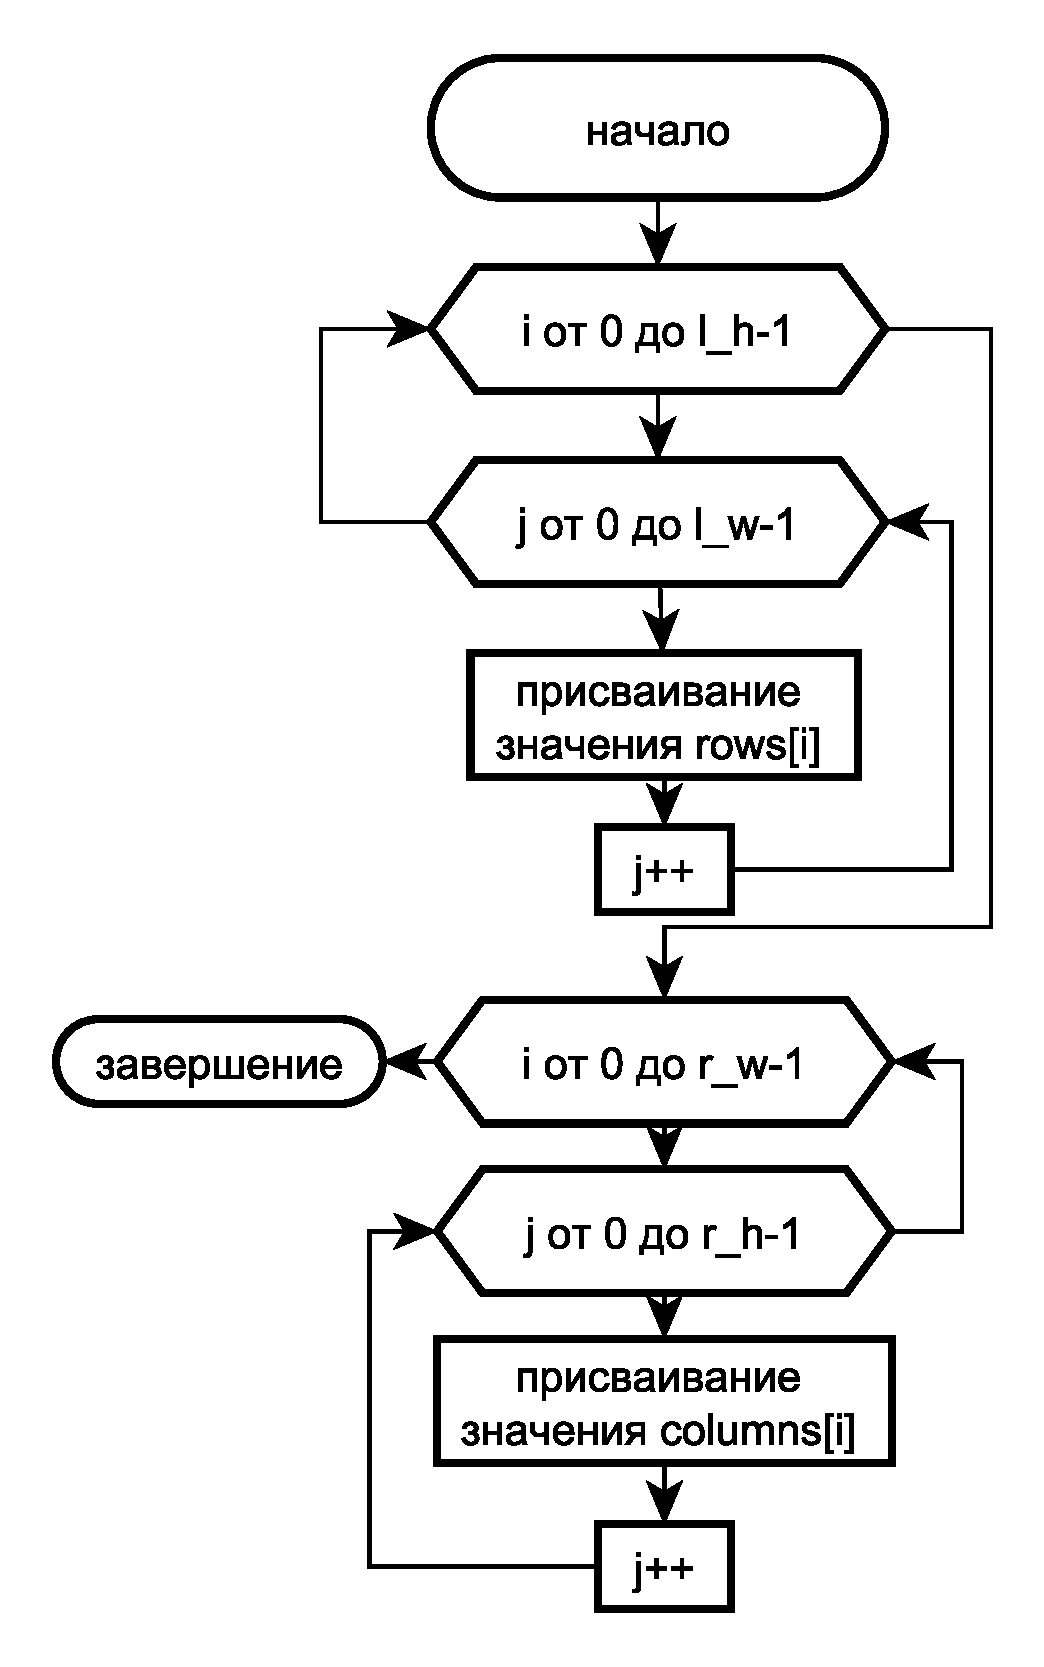
\includegraphics[width = 0.75\textwidth, height = 0.9\textheight]{flows_3}
		\captionof{figure}{PrepairArrays}
		\label{fig:label3}
		
		\includegraphics[width = 0.95\textwidth, height = 0.9\textheight]{diagram_4}
		\captionof{figure}{OptimizedPrepairArrays}
		\label{fig:label4}
		
		\includegraphics[width = 0.8\textwidth, height = 0.9\textheight]{diagram_5}
		\captionof{figure}{Алгоритм Винограда}
		\label{fig:label5}
		
		
		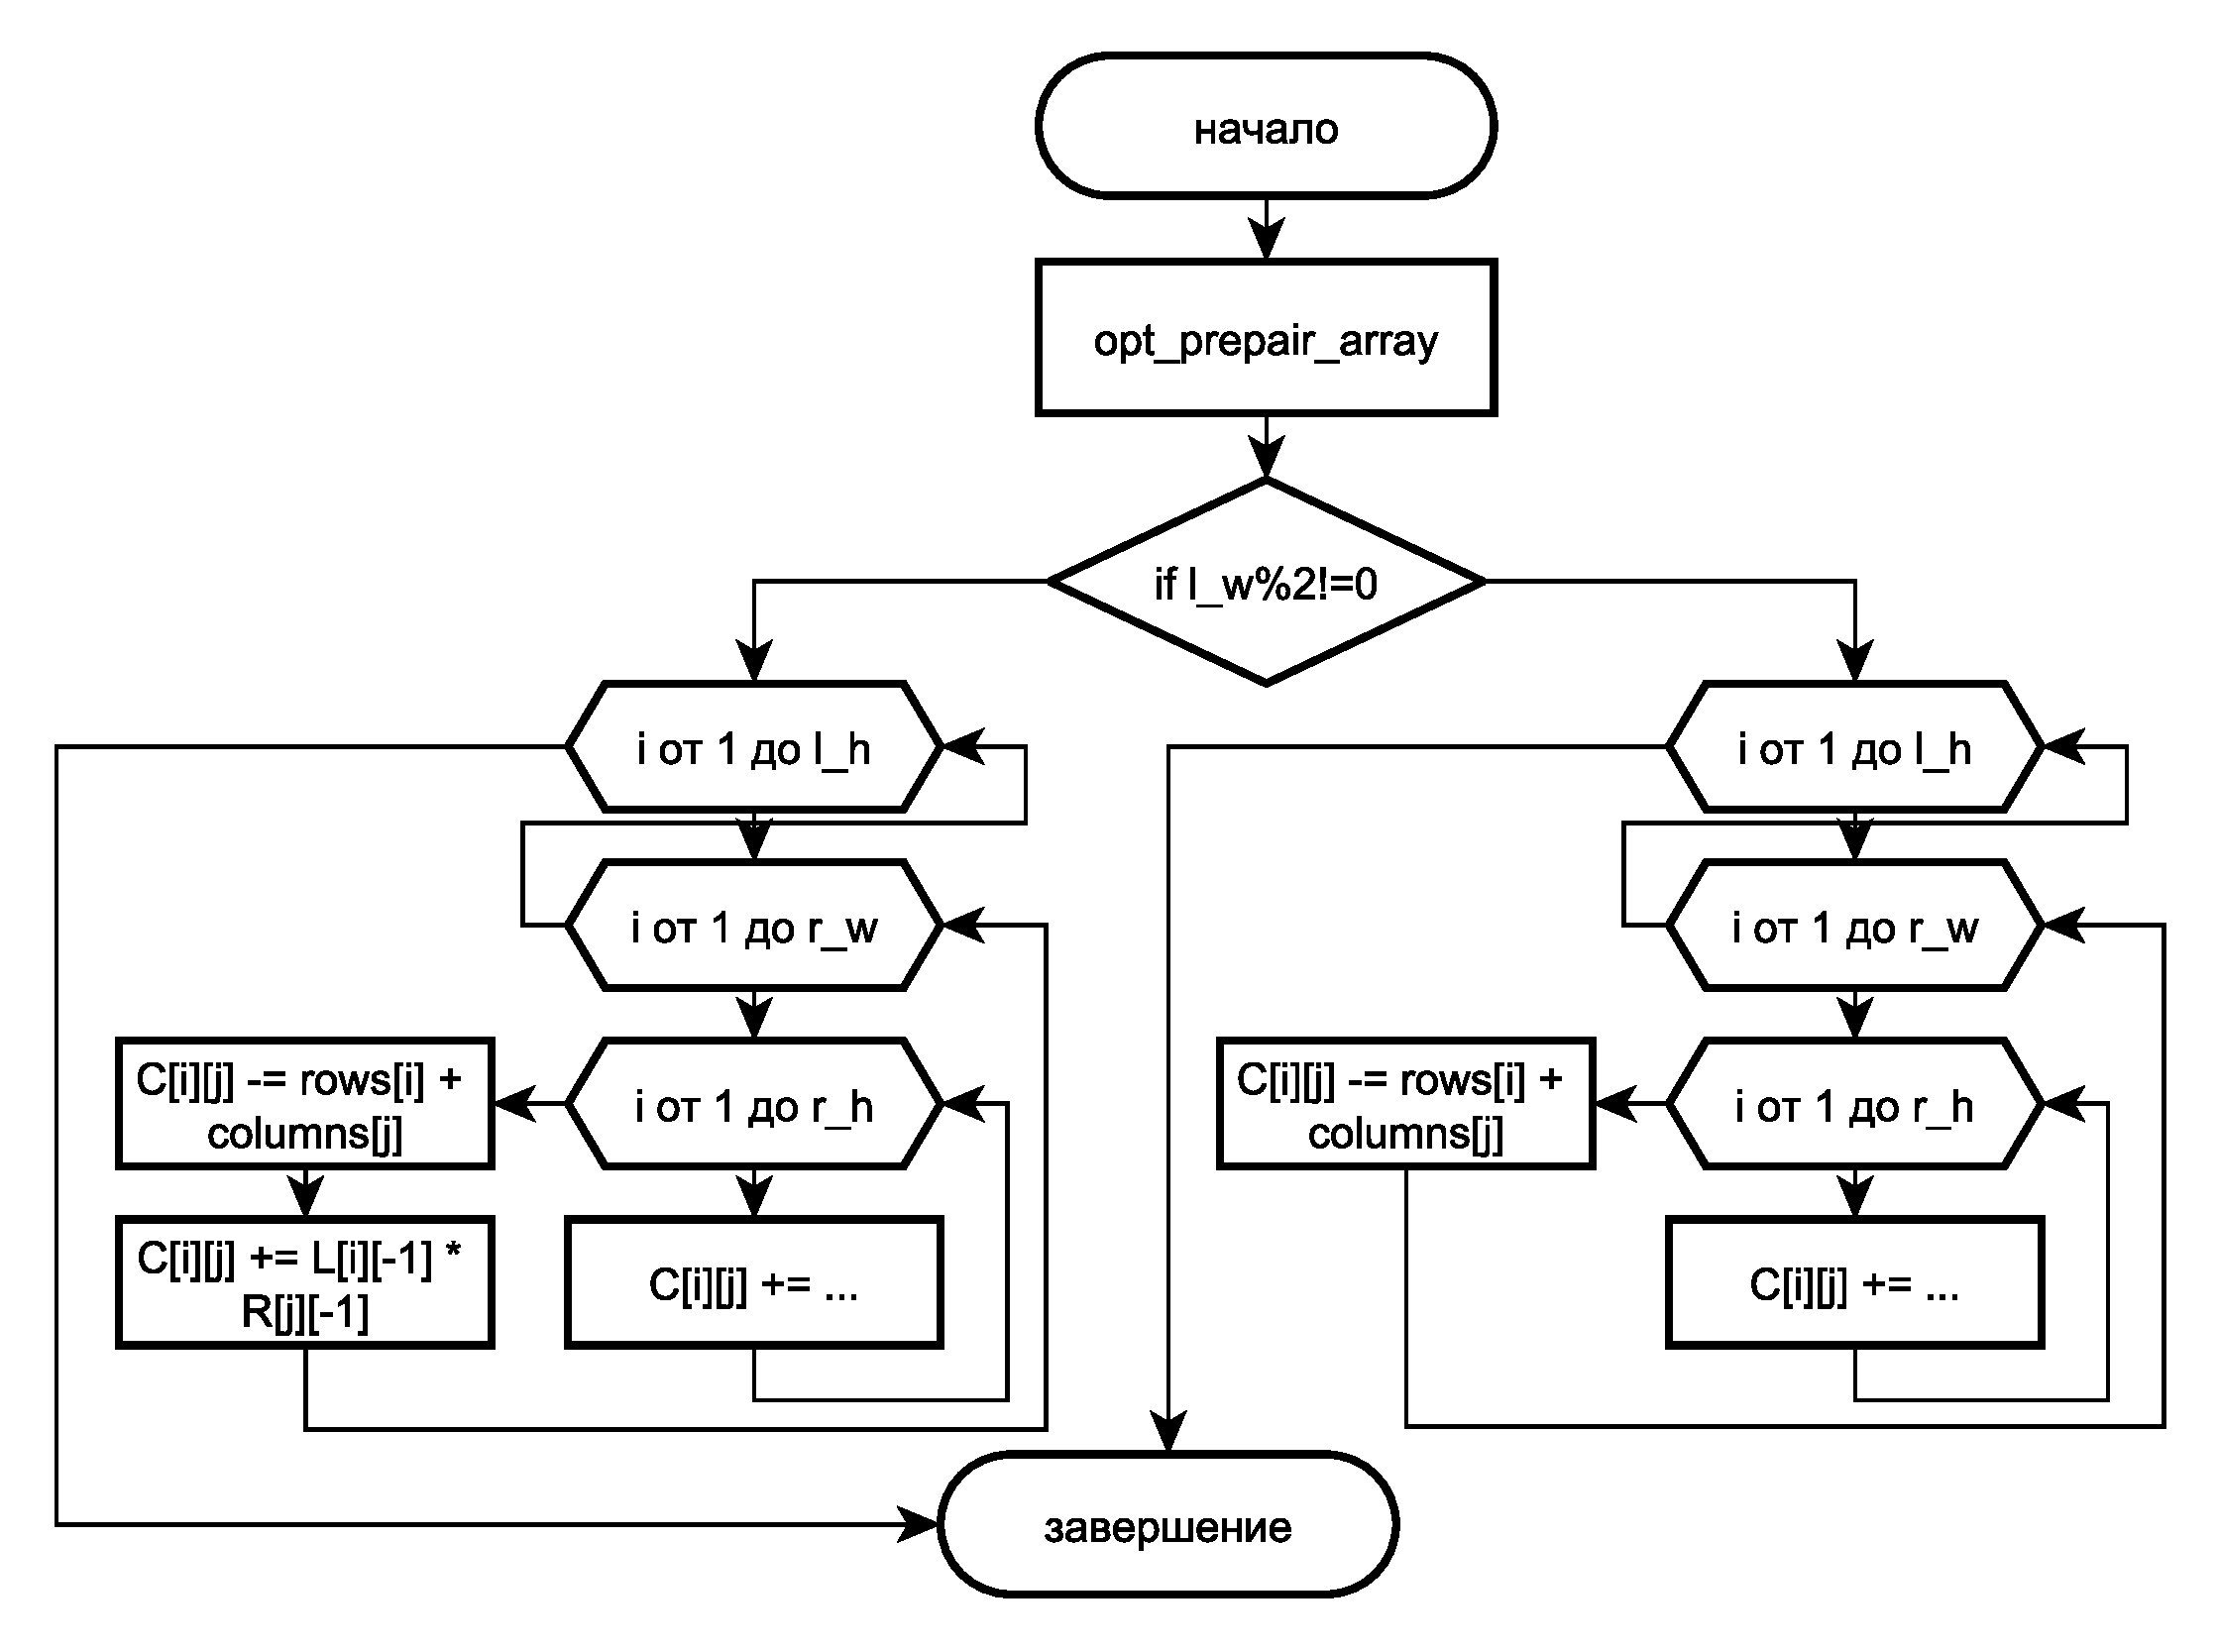
\includegraphics[width = 0.95\textwidth, height = 0.7\textheight]{diagram_6}
		\captionof{figure}{Оптимизированный Алгоритм Винограда}
		\label{fig:label6}
	\end{center}
	\newpage
	\subsection{Анализ сложностей} 
	Обычный(лучший случай, остальные случаи):
	\begin{equation*}
		\left[ 
		\begin{gathered} 
			0, lw \neq rh \\ 
			2 + 4\cdot lh + 4\cdot rw\cdot lh+14\cdot rw\cdot lw\cdot lh \\ 
		\end{gathered} 
		\right.
	\end{equation*}
	
	Стандартный алгоритм подготовки массивов rows и columns(prep\_arr)
	\begin{equation*}
		\left[ 
		\begin{gathered} 
			0, lw \neq rh \\ 
			2 + 4\cdot lh + 12\cdot rw\cdot lh \\
		\end{gathered} 
		\right.
	\end{equation*}
	
	Виноград(лучший случай, чётные матрицы, остальные случаи):
	\begin{equation*}
		\left[ 
		\begin{gathered} 
			0, lw \neq rh \\ 
			4 + 6\cdot lh + 12\cdot lw + 8\cdot rw\cdot lh + 27/2\cdot rw\cdot lh\cdot rh \\
			4 + 6\cdot lh + 12\cdot lw + 8\cdot rw\cdot lh + 9rw\cdot lh + 27/2\cdot rw\cdot lh\cdot rh \\
		\end{gathered} 
		\right.
	\end{equation*}
	
	Оптимизированный алгоритм подготовки массивов rows
	
	 columns(opt\_prep\_arr)
	\begin{equation*}
		\left[ 
		\begin{gathered} 
			0, lw \neq rh \\ 
			2 + lh + rw + 19*max + 2*max*lw + 9/2*lw*rh + 9/2*lw*rw\\
		\end{gathered} 
		\right.
	\end{equation*}
	Где max = max(lh, rw)
	
	Оптимизированный Виноград(лучший случай, чётные матрицы, остальные случаи):
	\begin{equation*}
		\left[ 
		\begin{gathered} 
			0, lw \neq rh \\ 
			6 + OptPrepArr + 4*lh + 10*rw*lh + 23/2*rw*rh*lh \\
			8 + OptPrepArr + 4*lh + 10*rw*lh + 7*rw*lh + 23/2*rw*rh*lh \\
		\end{gathered} 
		\right.
	\end{equation*}
	
	Стандартный алгоритм будет работать дольше всего в связи с тем, что коэфицент при rw*rh*lh (что является самой трудозатратной частью алгоритма при достаточно больших матрицах) в этом алгоритме больше чем в других (27/2 - Виноград и 23/2 оптимизированный Виноград) остальная часть играет меньшую роль в значении трудозатратности алгоритма.
	\par
	
	\newpage
	
	\section{Технологическая часть} 
	
	\subsection{Выбор средств реализации}
	Для программной реализации алгоритма использовалась среда разработки Visual Studio, язык программирования, на котором была выполнена реализации алгоритмов, --- C++. 
	Исследование проводилось на ноутбуке (64-разрядная операционная система, процессор x64, частота процессора 3.10~Ггц, оперативная память 16~ГБ)\par
	Для замера времени использовалась функция now() библиотеки chrono[\ref{s:2}].
	
	\subsection{Реализация алгоритмов}
	В листинге~\ref{list1} можно увидеть программную реализацию описанных алгоритмов.
	\lstset{
		language=C++,
		basicstyle=\ttfamily\fontsize{12}{14}\selectfont,
		breaklines=true,
		keywordstyle=\color{blue},
		commentstyle=\color{gray},
		stringstyle=\color{red},
		postbreak=\mbox{\textcolor{red}{$\hookrightarrow$}\space},
		showstringspaces=false,
		keepspaces=true,
		numbers=left,              
		numberstyle=\tiny,           
		stepnumber=1,                 
		numbersep=5pt,               
		backgroundcolor=\color{white},
		frame=single,  
	}
	
	\begin{lstlisting}[label = list1, caption = Программная реализация]	
template<class dtype>
Mass<dtype> multiplication(Mass<dtype>& array_l, Mass<dtype>& array_r) {
	Mass<dtype> new_ar(array_l.get_height(), array_r.get_wide());
	Timer x;
	x.start_time();
	for (int i = 0; i < array_l.get_height(); i++) {
		for (int j = 0; j < array_r.get_wide(); j++) {
			for (int k = 0; k < array_l.get_wide(); k++) {
				new_ar[i][j] += array_l[i][k] * array_r[k][j];
			}
		}
	}
	x.stop_time();
	x.get_time();
	return new_ar;
}

///////////////////vinograd///////////////////

template<class dtype>
void prepair_arrays(dtype* array_rows, dtype* array_columns, Mass<dtype>& array_l, Mass<dtype>& array_r, int l_h, int l_w, int r_h, int r_w) {
	
	for (int i = 0; i < l_h; i++) {
		array_rows[i] = 0;
		for (int j = 0; j < l_w; j++) {
			array_rows[i] += array_l[i][j] * array_l[i][j + 1];
			j++;
		}
	}
	array_rows[l_h] = -1;
	for (int i = 0; i < r_w; i++) {
		array_columns[i] = 0;
		for (int j = 0; j < r_h; j++) {
			array_columns[i] += array_r[j][i] * array_r[j + 1][i];
			j++;
		}
	}
	array_columns[r_w] = -1;
}

template<class dtype>
Mass<dtype> vinograd_multiplication(Mass<dtype>& array_l, Mass<dtype>& array_r) {
	Mass<dtype> new_ar(array_l.get_height(), array_r.get_wide());
	dtype fix_rows[FIX_ARR_SIZE];
	dtype fix_columns[FIX_ARR_SIZE];
	
	Timer x;
	x.start_time();
	
	BOOL A = TRUE;
	int l_h = array_l.get_height();
	int l_w = array_l.get_wide();
	int r_h = array_r.get_height();
	int r_w = array_r.get_wide();
	
	if ((array_l.get_wide() % 2) != 0) {
		A = FALSE;
		l_w -= 1;
		r_h -= 1;
	}
	
	
	prepair_arrays(fix_rows, fix_columns, array_l, array_r, l_h, l_w, r_h, r_w);
	
	for (int i = 0; i < l_h; i++) {
		for (int j = 0; j < r_w; j++) {
			for (int k = 0; k < (r_h); k++) {
				new_ar[i][j] += (array_l[i][k] + array_r[(k) + 1][j]) * (array_l[i][(k) + 1] + array_r[(k)][j]);
				k++;
			}
			if (!(A)) {
				new_ar[i][j] += array_l[i][l_w] * array_r[r_h][j];
			}
			new_ar[i][j] -= (fix_rows[i] + fix_columns[j]);
		}
	}
	
	x.stop_time();
	x.get_time();
	
	return new_ar;
}

///////////////////optimized_vin///////////////////

template<class dtype>
void opt_prepair_arrays(dtype* array_rows, dtype* array_columns, Mass<dtype>& array_l, Mass<dtype>& array_r, int l_h, int l_w, int r_h, int r_w) {
	int lim = max(l_h, r_w);
	int counter = 0;
	bool L = true;
	bool R = true;  
	while (counter < lim) {
		if (L) {
			array_rows[counter] = 0;
		}
		if (R) {
			array_columns[counter] = 0;
		}
		if ((l_w != 1) && (l_h != 1)) {
			array_rows[counter] += array_l[counter][0] * array_l[counter][1];
			array_columns[counter] += array_r[0][counter] * array_r[1][counter];
		}
		for (int j = 1; j < (l_w / 2); j++) {
			if (L) {
				array_rows[counter] += array_l[counter][j << 1] * array_l[counter][(j << 1) + 1];
			}
			if (R) {
				array_columns[counter] += array_r[j << 1][counter] * array_r[(j << 1) + 1][counter];
			}
		}
		counter++;
		if (counter >= l_h) L = false;
		if (counter >= r_w) R = false;
	}
	array_rows[l_h] = -1;
	array_columns[r_w] = -1;
}


template<class dtype>
Mass<dtype> optimized_vinograd_multiplication(Mass<dtype>& array_l, Mass<dtype>& array_r) {
	Mass<dtype> new_ar(array_l.get_height(), array_r.get_wide());
	dtype fix_rows[FIX_ARR_SIZE];
	dtype fix_columns[FIX_ARR_SIZE];
	
	Timer x;
	x.start_time();
	
	bool A = true;
	int l_h = array_l.get_height();
	int l_w = array_l.get_wide();
	int r_h = array_r.get_height();
	int r_w = array_r.get_wide();
	
	
	if ((array_l.get_wide() % 2) != 0) {
		A = FALSE;
		l_w -= 1;
		r_h -= 1;
	}
	
	opt_prepair_arrays(fix_rows, fix_columns, array_l, array_r, l_h, l_w, r_h, r_w);
	if (!(A)) {
		for (int i = 0; i < l_h; i++) {
			for (int j = 0; j < r_w; j++) {
				for (int k = 0; k < (r_h / 2); k++) {
					new_ar[i][j] += (array_l[i][k << 1] + array_r[(k << 1) + 1][j]) * (array_l[i][(k << 1) + 1] + array_r[(k << 1)][j]);
				}
				new_ar[i][j] -= (fix_rows[i] + fix_columns[j] - array_l[i][l_w] * array_r[r_h][j]);
			}
		}
	}
	else {
		for (int i = 0; i < l_h; i++) {
			for (int j = 0; j < r_w; j++) {
				for (int k = 0; k < (r_h / 2); k++) {
					new_ar[i][j] += (array_l[i][k << 1] + array_r[(k << 1) + 1][j]) * (array_l[i][(k << 1) + 1] + array_r[(k << 1)][j]);
				}
				new_ar[i][j] -= (fix_rows[i] + fix_columns[j]);
			}
		}
	}
	
	x.stop_time();
	x.get_time();
	
	return new_ar;
}

///////////////////MODES///////////////////

void MODE_1() {
	int hei, wid;
	cout << "write height and wide for first" << "\n";
	cin >> hei;
	cin >> wid;
	Mass<int> A(hei, wid);
	Mass<int> C;
	cout << "fill the first matrix" << "\n";
	A.fill_arr(1);
	A.print();
	cout << "write height and wide for second" << "\n";
	cin >> hei;
	cin >> wid;
	Mass<int> B(hei, wid);
	cout << "fill the second matrix" << "\n";
	B.fill_arr(1);
	cout << "Ordinary:\n";
	C = multiplication(A, B);
	C.print();
	C = vinograd_multiplication(A, B);
	cout << "Vinograd:\n";
	C.print();
	cout << "Optimized Vingrad:\n";
	C = optimized_vinograd_multiplication(A, B);
	C.print();
}


void MODE_2() {
	srand(time(0));
	int size;
	
	for (int i = 0; i < 10; i++) {
		size = 10 + 10 * i;
		cout << "SIZE: " << size << endl;
		Mass<int> A(size, size);
		Mass<int> B(size, size);
		Mass<int> C(size, size);
		for (int r = 0; r < size; r++) {
			for (int c = 0; c < size; c++) {
				A[r][c] = get_num();
				B[r][c] = get_num();
			}
		}
		cout << "-----A*B----- ";
		C = multiplication(A, B);
		cout << "-----A*B_vin----- ";
		C = vinograd_multiplication(A, B);
		cout << "-----A*B_opt_vin----- ";
		C = optimized_vinograd_multiplication(A, B);
	}
}
\end{lstlisting}
	
\newpage
\subsection{Тестирование программы}

В таблицах~\ref{tab:tests} и ~\ref{tab:tests2} представлены описания тестов по методологии чёрного ящика, все тесты пройдены успешно
Все тесты пройдены успешно.

\begin{table}[htbp]
	\caption{Асимптотические сложности реализаций алгоритмов}
	\centering
	\begin{tabular}{|p{0.05\linewidth}|p{0.2\linewidth}|p{0.12\linewidth}|p{0.25\linewidth}|p{0.25\linewidth}|}
		\hline
		& \textbf{Описание теста} & \textbf{Входные данные} & \textbf{Ожидаемый результат} & \textbf{Полученный результат} \\
		\hline
		
		\textbf{1} & проверка на обработку не валидных данных & 1 2 \newline 3 \newline 3 \newline 3 1 & оповещение о некорректности данных и запрос новых & оповещение о некорректности данных и запрос новых \\
		\hline
		
		\textbf{2} & проверка на обработку нулевой матрицы & 0 1&оповещение программы и запрос новых данных&оповещение программы и запрос новых данных\\
		\hline
		
		\textbf{3} & умножение квадратных матриц & 2 2\newline 
		1\newline 2\newline 3\newline 4\newline 2 2\newline 
		5\newline 6\newline 7\newline 8\newline& 19 22 \newline 43 50
		& 19 22 \newline 43 50\\
		\hline
		
	\end{tabular}
	\label{tab:tests}
\end{table}

\begin{table}[htbp]
	\caption{Асимптотические сложности реализаций алгоритмов}
	\centering
	\begin{tabular}{|p{0.05\linewidth}|p{0.2\linewidth}|p{0.12\linewidth}|p{0.25\linewidth}|p{0.25\linewidth}|}
		\hline
		
		\textbf{4} & умножение не квадратных матриц & 1 2\newline 
		1\newline 2\newline 2 3\newline 5 \newline 6 \newline 7 \newline 8 \newline 9 \newline 10& 21 24 27 \newline 47 54 61
		& 21 24 27 \newline 47 54 61\\
		\hline
		
		\textbf{5} & умножение векторов & 1 2\newline 
		1\newline 2\newline 2 1\newline 5 \newline 6& 17
		& 17\\
		\hline
		
	\end{tabular}
	\label{tab:tests2}
\end{table}
\clearpage	

\section{Исследовательская часть}
\subsection{Графики зависимостей процессорного времени}
В результате работы был проведён массированный замер эффективности реализаций алгоритмов. В результате этого замера, составлен график зависимости процессорного времени от размера перемножаемых матриц. График изображён на рисунке ~\ref{grh:1}.

	
	\includegraphics[width = 0.8\textwidth, height = 0.3\textheight]{chart_1}
	\captionof{figure}{Визуализация зависимости процессорного времени выполнения алгоритмов от размеров матриц}
	\label{grh:1}
	

Из этого можно сделать вывод, что реализация алгоритма Винограда и оптимизированного алгоритма Винограда затрачивают меньше процессорного времени для расчёта сответствующих матриц. Но они используют большее количество памяти, так как помимо трёх двумерных массивов (матриц) должны хранить ещё и два массива со значаниями часто используемых произведений .\par

\newpage
\section*{ЗАКЛЮЧЕНИЕ}
\addcontentsline{toc}{section}{ЗАКЛЮЧЕНИЕ}


В результате лабораторной работы была достигнута цель -- рассмотрены и разобраны три алгоритма перемножения матриц (стандартный, Виноград, оптимизированный Виноград).

Были выполнены все поставленные задач.
\begin{enumerate}
	\item Описана математическая основу обычного алгоритма, алгоритма Винограда и оптимизированного алгоритма Винограда перемножения стриц,
	\item Описана модель вычисления,
	\item Реализована программа на основе этих алгоритмов,
	\item Выполнена оценка трудоёмкости реализации алгоритмов,
	\item Реализованы разработанные алгоритмы в программном обеспечении с 2-мя режимами работы -- одиночного расчёта и массированного замера процессорного времени,
	\item Выполнены замеры процессорного времени выполнения реализации каждого алгоритма в зависимости от размера матриц,
	\item Выполнен сравнительный анализ рассчитанных трудоёмкостей и результатов замера процессорного времени,
\end{enumerate}

\newpage
\section*{СПИСОК ИСПОЛЬЗОВАННЫХ ИСТОЧНИКОВ}

\addcontentsline{toc}{section}{СПИСОК ИСПОЛЬЗОВАННЫХ ИСТОЧНИКОВ}
\begin{list}{\arabic{enumi}.}{\usecounter{enumi} \leftmargin=0pt \rightmargin=0pt}
	\item \justifying Ульянов М. В. Ресурсно эффективные компьютерные алгоритмы. Москва 2007. ФИЗМАТЛИТ. 376 стр.\label{s:1}
	
	\item \justifying Microsoft. GetProcessTimes function. [Электронный ресурс] - URL:https://learn.microsoft.com/ru-ru/cpp/standard-library/processthreadsapi/chrono \par
	(дата обращения: 20.09.2024).\label{s:2}
	
	\item \justifying AlgoLib. [Электронный ресурс] - URL: https://www.algolib.narod/Math/Matrix \par
	(дата обращения: 20.09.2024).\label{s:3}
\end{list}
	
\end{document}

